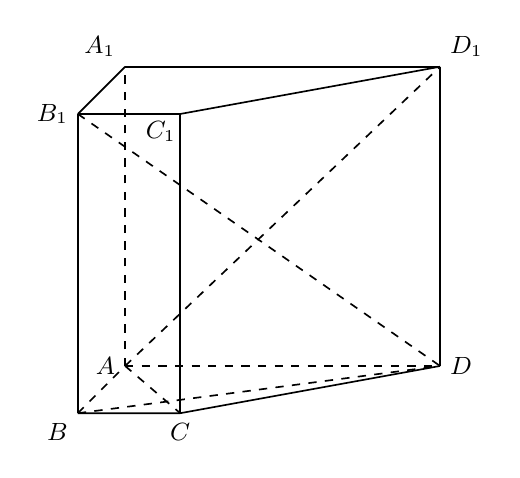
\begin{tikzpicture}[line width=.6pt, font=\small, >=stealth]
\coordinate (A) at (0.6,0.6);
\coordinate (B) at (0,0);
\coordinate (C) at (1.3000000000,0.0000000000);
\coordinate (D) at (4.6,0.6);
\coordinate (A1) at (0.6,4.4);
\coordinate (B1) at (0,3.8);
\coordinate (C1) at (1.3000000000,3.8000000000);
\coordinate (D1) at (4.6,4.4);
% bottom face
\draw[dashed] (A)--(D);
\draw (B)--(C)--(D);
\draw[dashed] (B)--(A);
\draw[dashed] (A)--(C);
\draw[dashed] (B)--(D);
% verticals
\draw (B)--(B1);
\draw (C)--(C1);
\draw (D)--(D1);
\draw[dashed] (A)--(A1);
% top face
\draw (A1)--(D1);
\draw (B1)--(C1);
\draw (B1)--(A1);
\draw (C1)--(D1);
% diagonals for proof (as in original)
\draw[dashed] (B1)--(D);
\draw[dashed] (A)--(D1);
\node[below left] at (B) {$B$};
\node[below] at (C) {$C$};
\node[right] at (D) {$D$};
\node[left] at (A) {$A$};
\node[left] at (B1) {$B_{1}$};
\node[below,xshift=-7pt,yshift=1pt] at (C1) {$C_{1}$};
\node[above left] at (A1) {$A_{1}$};
\node[above right] at (D1) {$D_{1}$};
\end{tikzpicture}
